\chapter{Resultados e Discussão}
\label{cap:04}

\section{Análise Qualitativa para Comparação entre \textit{Kotlin} e \textit{Java}}

Neste capítulo, apresenta-se análise a respeito do desempenho de cada uma das linguagens analisadas em âmbito geral, levando em consideração cada um dos experimentos em \textit{Kotlin} e \textit{Java}, desenvolvidos na seção anterior. 

\subsection{Comparação das Métricas}

Ao decorrer da presente seção, serão apresentados índices baseados no artigo: Análise Comparativa de Linguagens de Programação a partir de Problemas Clássicos da Computação, publico na revista Revista de Sistemas e Computação - RSC, desenvolvido na Universidade Federal de Itajubá do estado de Minas Gerais, no qual se estabelece um estudo comparativo sobre o tamanho dos algoritmos, velocidade de execução e tamanho em \textit{bytes} entre \textit{C}, \textit{Java} e \textit{Python}, ambas linguagens que encontram-se sempre no topo de pesquisas de popularidade. O estudo foi realizado por meio de experimentos matemáticos com diversas fórmulas amplamente conhecidas, os autores concluem com base nas comparações desenvolvidas, que a linguagem \textit{C} possui mais características para ser a escolhida.

Com o intuito de se estabelecer indicadores de qualidade, a fim de se efetuar uma avaliação referente aos algoritmos apresentados nos experimentos I, II, III, IV, V, VI e VII, foram definidos, como base, três índices qualificadores para avaliação, sendo eles:

\begin{itemize}
    \item Índice \textbf{A} (satisfatório): Implementação de algoritmo que realiza a utilização de poucos caracteres especiais, símbolos, assim como baixa quantidade de linhas de código;
     \item Índice \textbf{B} (parcialmente satisfatório): Implementação de algoritmo que se utiliza de mais caracteres especiais, símbolos ou maior quantidade de linhas de código;
      \item Índice \textbf{C} (insatisfatório): Implementação de algoritmo que se utiliza de maior quantidade de caracteres especiais, símbolos e linhas de código.
\end{itemize}

De acordo com os índices de qualidade exemplificados a seguir na Tabela 4, apresentam-se as métricas referentes aos códigos desempenhados no decorrer do capítulo 4:

\FloatBarrier
\begin{table}[!htbp]
\centering
\caption{Métrica Geral dos Experimentos}
	\begin{tabular}{ c | c | c }
		\hline
        \textbf{Métrica} &  \textbf{\textit{Kotlin}}    & \textbf{\textit{Java}}  \\ \hline
		
		  Caracteres utilizados   &     A 	       &            B     \\ \hline
		             
		  Linhas de código        &     A          &            B       \\ \hline
		             
		  Tamanho em \textit{bytes}        &     A          &            A      \\ \hline
		  
	\end{tabular}
	\\ \vspace{0.2cm}
	\textbf{Fonte:} Elaborada pelo autor
	\label{tab:exemplo}
\end{table}
\FloatBarrier

Conforme apresentado na Tabela 4, sobre a linguagem \textit{Kotlin} baseando-se unicamente nos algoritmos implementados e na formatação utilizada, facilita a menor utilização de caracteres especiais, símbolos e linhas de código, em comparação com a linguagem de programação \textit{Java}, recebendo assim, o índice de qualidade A em todos os quesitos analisados, levando em consideração os experimentos de introdução, sendo eles: I - \textit{Hello World}, II - operação aritmética de soma e III - classe \textit{Student}, também como os experimentos que demonstraram a implementação de aplicação de conversão de medidas termométricas, sendo eles:  IV - classe \textit{ThermometricScale}, V - interface \textit{Temperature}, VI - classe \textit{Adapter} e VII - classe \textit{Activity Main}.

\subsection{Pontos Positivos e Negativos da Adoção do Kotlin}

No ato de integrar-se em um projeto já existente, a compatibilidade com a linguagem de programação \textit{Kotlin}, observa-se um aumento de alguns segundos no tempo de execução da aplicação, e em caso de uma aplicação escrita somente em \textit{Kotlin}, o tempo de execução também é maior se comparada a uma aplicação desenvolvida em \textit{Java}. Por mais que seja possível literalmente misturar códigos em \textit{Java} e \textit{Kotlin} no mesmo projeto e até no mesmo arquivo, observa-se que para aproveitar-se todos os recursos oferecidos pela nova linguagem, como tornar o código mais enxuto e aumentar sua flexibilidade, necessita-se de consultas e estudos a documentação, uma vez que o recurso de conversão de \textit{Java} para \textit{Kotlin} que é disponibilizado nativamente pela \textit{IDE Android Studio} em versões mais recentes e por meio de \textit{plugins} em versões anteriores, não realiza a conversão da forma mais enxuta e direta possível, mas sim da forma mais verbosa, como por exemplo, a não utilização do recurso de importação de todos os \textit{widgets} utilizados no arquivo \textit{XML} de \textit{layout}, conforme demonstrado no experimento VII \textit{activity main}. 

O fato de \textit{Kotlin} ser totalmente integrada com a \textit{IDE Android Studio} torna a sua utilização/adoção bem atrativa e descomplicada. A compatibilidade da linguagem com \textit{Java} torna o desenvolvimento mais leve, deixando a cargo do desenvolvedor, escolher qual sintaxe, estilo e padronização de escrita de código utilizar, como por exemplo optar por utilizar ponto e vírgula ao final de cada instrução (\textit{Java}) ou não (\textit{Kotlin}). A curva de aprendizado apresenta-se baixa para desenvolvedores com conhecimento prévio em \textit{Java} e nas particularidades do desenvolvimento móvel voltado para o dispositivos móveis e o ecossistema da plataforma \textit{Android}.

\section{Análise Quantitativa para Comparação entre \textit{Kotlin} e \textit{Java}}

Para efetuar a comparação entre as linguagens \textit{Java} e \textit{Kotlin}, utiliza-se ferramenta disponibilizada de forma gratuita no endereço \textit{web} \url{https://www.4devs.com.br/analisar_textos}, que realiza a funcionalidade de contabilização de caracteres, palavras e de linhas de código. Conforme apresentado na Figura 13 a seguir, após inserir o algoritmo a ser analisado, logo abaixo do campo de texto, apresentam-se os campos onde são disponibilizados os valores.

\FloatBarrier
\begin{figure*}[!htbp]
	\centering
		\caption{Ferramenta de contagem de caracteres, palavras e linhas}
	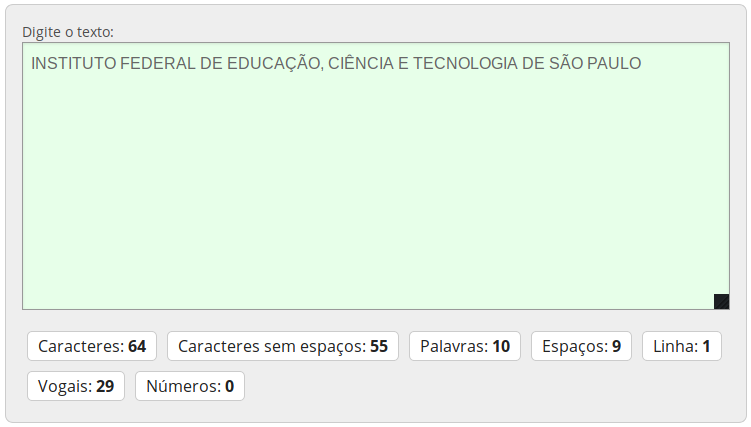
\includegraphics[scale=0.8]{imagens/4devs}
	\subcaption{\textbf{Fonte:} \url{https://www.4devs.com.br/analisar_textos}}
	\label{fig:figura3}
\end{figure*}
\FloatBarrier

Nas subseções posteriores, apresentam-se as tabelas com as devidas métricas de quantidade de caracteres, linhas de código e tamanho em \textit{bytes}, ambas as métricas obtidas por meio da disponibilização dos trechos de códigos utilizados nos experimentos, conforme demonstrado na Figura 13.

\subsection{Experimento I}

No exemplo de implementação de um simples e introdutório algoritmo de \textit{Hello World}, \textit{Kotlin} atingiu o objetivo, com uma menor quantidade de caracteres utilizados, linhas de código e consequentemente de \textit{bytes}, conforme Tabela 5 a seguir.

\FloatBarrier
\begin{table}[!htbp]
\centering
\caption{Métricas \textit{Hello World}}
	\begin{tabular}{ c | c | c }
		\hline
           \textbf{Métrica} &            \textbf{\textit{Kotlin}}    & \textbf{\textit{Java}}  \\ \hline
		
		  Caracteres utilizados   &     39 	           &             116     \\ \hline
		             
		  Linhas de código        &     03             &             05       \\ \hline
		             
		  Tamanho em \textit{bytes}        &     39             &             117      \\ \hline
		  
	\end{tabular}
	\\ \vspace{0.2cm}
	\textbf{Fonte:} Elaborada pelo autor
	\label{tab:exemplo}
\end{table}
\FloatBarrier

\subsection{Experimento II}

De acordo com a Tabela 6, no experimento de implementação de operação de soma, que retorna a soma de dois valores fixos e inteiros, interpolados com um pequeno trecho de texto, \textit{Kotlin} obteve os menores índices em todas as métricas analisadas.


\FloatBarrier
\begin{table}[!htbp]
\centering
\caption{Métricas Operação Aritmética de Soma}
	\begin{tabular}{ c | c | c }
		\hline
          \textbf{Métrica} &          \textbf{\textit{Kotlin}}    & \textbf{\textit{Java}}  \\ \hline
		
		  Caracteres utilizados   &     81 	           &            159      \\ \hline
		             
		  Linhas de código        &     5             &            6      \\ \hline
		             
		  Tamanho em \textit{bytes}        &     80             &           159      \\ \hline
		  
	\end{tabular}
	\\ \vspace{0.2cm}
	\textbf{Fonte:} Elaborada pelo autor
	\label{tab:exemplo}
\end{table}
\FloatBarrier

\subsection{Experimento III}

No experimento de implementação de uma classe que abstrai de maneira simples, as características de um estudante, \textit{Kotlin} demonstra a possibilidade de evitar códigos desnecessários em algoritmos comumente utilizados, possibilitando a economia de mais de mil caracteres e 60 linhas de implementação, conforme Tabela 7. 

\FloatBarrier
\begin{table}[!htbp]
\centering
\caption{Métricas Classe \textit{Student}}
	\begin{tabular}{ c | c | c }
		\hline
          \textbf{Métrica} &          \textbf{\textit{Kotlin}}    & \textbf{\textit{Java}}  \\ \hline
		
		  Caracteres utilizados   &     163 	      &          1.607      \\ \hline
		             
		  Linhas de código        &     4             &            67      \\ \hline
		             
		  Tamanho em \textit{bytes}        &     163           &          1.600     \\ \hline
		  
	\end{tabular}
	\\ \vspace{0.2cm}
	\textbf{Fonte:} Elaborada pelo autor
	\label{tab:exemplo}
\end{table}
\FloatBarrier

\subsection{Experimento IV}

Com a implementação da classe \textit{ThermometricScale}, de acordo com a Tabela 8, observa-se por meio da implementação da declaração de funções, parâmetros e seus respectivos retornos disponível em \textit{Kotlin}, economiza-se diversas linhas de código, podendo variar de acordo com a abordagem do(s) desenvolvedor(s).

\FloatBarrier
\begin{table}[!htbp]
\centering
\caption{Métricas Classe \textit{ThermometricScale}}
	\begin{tabular}{ c | c | c }
		\hline
          \textbf{Métrica} &          \textbf{\textit{Kotlin}}    & \textbf{\textit{Java}}  \\ \hline
		
		  Caracteres utilizados   &     283 	      &          363      \\ \hline
		             
		  Linhas de código        &     9             &           16      \\ \hline
		             
		  Tamanho em \textit{bytes}        &     285           &          364      \\ \hline
		  
	\end{tabular}
	\\ \vspace{0.2cm}
	\textbf{Fonte:} Elaborada pelo autor
	\label{tab:exemplo}
\end{table}
\FloatBarrier

\subsection{Experimento V}

No experimento no qual implementa-se a função da interface \textit{Temperature} a ser implementada, \textit{Kotlin} e \textit{Java} utilizam a mesma quantidade de linhas de código, \textit{Kotlin} obtém os resultados menores na métrica de caracteres utilizados e tamanho em \textit{bytes}, conforme Tabela 9.

\FloatBarrier
\begin{table}[!htbp]
\centering
\caption{Métricas Interface \textit{Temperature}}
	\begin{tabular}{ c | c | c }
		\hline
          \textbf{Métrica} &         \textbf{\textit{Kotlin}}    & \textbf{\textit{Java}}  \\ \hline
		
		  Caracteres utilizados   &     143 	      &          155      \\ \hline
		             
		  Linhas de código        &     5             &           5      \\ \hline
		             
		  Tamanho em \textit{bytes}        &     144           &          156      \\ \hline
		  
	\end{tabular}
	\\ \vspace{0.2cm}
	\textbf{Fonte:} Elaborada pelo autor
	\label{tab:exemplo}
\end{table}
\FloatBarrier

\subsection{Experimento VI}

De acordo com a Tabela 10, na implementação da classe que tem por objetivo ser um adaptador no aplicativo de conversão, demonstra-se que Java necessita de maiores quantidades de linhas de código, caracteres e um tamanho superior em \textit{bytes}.

\FloatBarrier
\begin{table}[!htbp]
\centering
\caption{Métricas Classe \textit{Adapter}}
	\begin{tabular}{ c | c | c }
		\hline
            \textbf{Métrica} &         \textbf{\textit{Kotlin}}    & \textbf{\textit{Java}}  \\ \hline
		
		  Caracteres utilizados   &     605 	      &          741      \\ \hline
		             
		  Linhas de código        &     19            &           26      \\ \hline
		             
		  Tamanho em \textit{bytes}        &     608           &          742      \\ \hline
		  
	\end{tabular}
	\\ \vspace{0.2cm}
	\textbf{Fonte:} Elaborada pelo autor
	\label{tab:exemplo}
\end{table}
\FloatBarrier

\subsection{Experimento VII}

Na classe principal do programa de conversão de Celsius para Fahrenheit e Kelvin, de acordo com a implementação utilizada, \textit{Java} demonstra a necessidade da utilização de mais caracteres, aumentando a quantidade de linhas de código , consequentemente, o tamanho em \textit{bytes}, conforme Tabela 11.

\FloatBarrier
\begin{table}[!htbp]
\centering
\caption{Métricas Classe \textit{Activity Main}}
	\begin{tabular}{ c | c | c }
		\hline
            \textbf{Métrica} &        \textbf{\textit{Kotlin}}    & \textbf{\textit{Java}}  \\ \hline
		
		  Caracteres utilizados   &     2.404 	      &          3.179      \\ \hline
		             
		  Linhas de código        &     74            &           93      \\ \hline
		             
		  Tamanho em \textit{bytes}        &     3.200           &          3.800      \\ \hline
		  
	\end{tabular}
	\\ \vspace{0.2cm}
	\textbf{Fonte:} Elaborada pelo autor
	\label{tab:exemplo}
\end{table}
\FloatBarrier